\section{Proof of concept: Weakly Connected Components of a Graph}\label{prole}

One of the biggest challenges of implementing a Dynamic Pipeline is to find  a programming language with a proper set of tools supporting both of the  primary features of the \acrshort{dp}: \begin{inparaenum}[i\upshape)]
\item  \emph{parallel} processing and 
\item  \emph{strong theoretical} foundations to manage computations as first-class citizens.
 \end{inparaenum}
Haskell is a statically typed pure functional language designed on strong theoretical foundations where computations are primary entities.
This pure functional language has evolved from its birth in 1987 and nowadays provides a powerful set of tools for writing multithreading and parallel programs with optimal performance \cite{parallelbook, monadpar}. 

In the context of this research, we first assessed the suitability of \acrlong{hs}  to implement a Dynamic Pipeline. 
To be concrete, we conducted a proof of concept implementing a Dynamic Pipeline in  Haskell for solving a particular and very relevant problem as the computation/enumeration of the Weakly Connected Components of a graph.
In particular, the main objective of our proof of concept was to study the critical features required in \acrshort{hs} for a \acrshort{dpf} implementation,  the real possibilities of emitting incrementally results, and the performance of such kinds of implementations. 
Indeed, we explored the basis of an implementation of a \acrshort{dpf}  in a pure (parallel) functional language as Haskell.
This is, we determined the particular features (i.e., versions and libraries) that will allow for an efficient implementation of a \acrshort{dpf}. 
Moreover, we conducted an empirical evaluation to analyze the performance of the Dynamic Pipeline implemented in Haskell for enumerating \acrshort{wcc} with special attention to the emission of results, i.e. \acrshort{wcc}, incrementally. 
In this chapter, we focus on the presentation of our algorithm for enumerating \acrshort{wcc} using \acrshort{hs} as well as the results obtained in the empirical evaluation of its implementation. 
 
\subsection{$\dpwcc$ Algorithm}
Let us consider the problem of computing/enumerating the (weak) connected components of a graph $G$ using \acrshort{dp}. 
A connected component of a graph is a subgraph in which any two vertices are connected by paths.  
Thus, finding connected components of an undirected graph implies obtaining the minimal partition of the set of nodes induced by the relationship \textit{connected}, i.e., there is a path between each pair of nodes. An example of that graph can be seen in \autoref{fig:example_dp_graph}.
The input of the Dynamic Pipeline for computing the WCC of a graph, $\dpwcc$, is a sequence of edges ending with $\eof$\footnote{Note that there are neither isolated vertices nor loops in the source graph $G$.}. The connected components are output as soon as they are computed, i.e., they are produced incrementally. 
Roughly speaking the idea of the algorithm is that the weakly connected components are built in two phases. In the first phase filter instance stages receive the edges of the input graph and create sets of connected vertices. 
During the second phase, these filter instances construct maximal subsets of connected vertices, i.e. the vertices corresponding to (weakly) connected components.
%
$\dpwcc$ is defined in terms of the behavior of its four kinds stages: \textit{Source} ($\iwc$),  \textit{Generator} ($\gwc$),  \textit{Sink} ($\owc$), and \textit{Filter}($\fwc$) stages. Additionally,  the channels connecting these stages must be defined. 
In $\dpwcc$, stages are connected linearly and unidirectionally through the channels $\ice$ and  $\csofv$. Channel $\ice$ carries edges while channel  $\csofv$ conveys sets of connected vertices. Both channels end by the $\eof$ mark. 
The behavior of $\fwc$ is given by a sequence of two actors (scripts). Each actor corresponds to a phase of the algorithm. In what follows, we denote these actors by $\Act$ and $\Actt$, respectively. 
The script $\Act$ keeps a set of connected vertices ($CV$) in the state of the $\fwc$ instance. When an edge $e$ arrives, if an endpoint of $e$ is present in the state, then the other endpoint of $e$ is added to $CV$. 
Edges without incident endpoints are passed to the next stage. When $\eof$ arrives at channel $\ice$, it is passed to the next stage, and the script $\Actt$ starts its execution. 
If script $\Actt$ receives a set of connected vertices $CV$ in $\csofv$, it determines if the intersection between $CV$ and the nodes in its state is not empty. If so, it adds the nodes in $CV$  to its state. 
Otherwise, the $CV$ is passed to the next stage.  Whenever $\eof$ is received, $\Actt$ passes--through $\csofv$-- the set of vertices in its state and the $\eof$ mark to the next stage; then, it dies.
The behavior of $\iwc$ corresponds to the identity transformation over the data stream of edges.  As edges arrive, they are passed through  $\ice$ to the next stage. When receiving $\eof$ on $\ice$, this mark is put on both channels. 
Then, $\iwc$ dies. 

%\begin{wrapfigure}{r}{0.4\textwidth}
\begin{figure}
 \begin{center}
\inputtikz{graph_example_wcc}
\end{center}
\caption[{[PoC] Graph WCC Example}]{Example of a graph with two weakly connected components: $\{1,2\}$ and $\{3,4,5,6\}$}
\label{fig:example_dp_graph}
\end{figure}
%\end{wrapfigure}

Let us describe this behavior with the example of the graph shown in \autoref{fig:example_dp_graph}.

\begin{figure}[h!]
  \centering
\inputtikz{dp_example_0}
\caption[{[PoC] $\dpwcc$ Initial Setup}]{$\dpwcc$ Initial setup. Stages Source, Generator, and Sink are represented by the squares labeled by $\mathsf{Sr_{WCC}}$, $\mathsf{G_{WCC}}$ and $\mathsf{Sk_{WCC}}$, respectively.  The square $\fwc$ corresponding to the Filter stage template is the parameter of $\gwc$. Arrows $\rightrightarrows$ between represents the connection of stages through two channels, $\ice$, and $\csofv$. The arrow  $\rightarrow$ represents the channel $\csofv$ connecting the stages $\mathsf{G_{WCC}}$ and $\mathsf{Sk_{WCC}}$. The arrow $\Longrightarrow$ stands for I/O data flow. Finally, the input stream comes between the dotted lines on the left and the WCC computed incrementally will be placed between the solid lines on the right.}
\label{fig:dp_example_0}
\end{figure}

\autoref{fig:dp_example_0} depicts the initial configuration of $\dpwcc$. 
The interaction of $\dpwcc$ with the "external" world is done through the stages $\iwc$ and $\owc$. 
Indeed, once activated the initial $\dpwcc$, the input stream -- consisting of a sequence containing all the edges in the graph in \autoref{fig:example_dp_graph} -- feeds $\iwc$ while  $\owc$ emits incrementally the resulting weakly connected components.  
In what follows \autoref{fig:dp_example_1_2}, \autoref{fig:dp_example_3_4}, \autoref{fig:dp_example_5_6}, \autoref{fig:dp_example_7_8} and \autoref{fig:dp_example_9_10} depict the evolution of the $\dpwcc$.
 
\begin{figure}[h!]
\centering
\begin{subfigure}[b]{\textwidth}
 \centering
  \inputtikz{dp_example_1}
  \caption{The edge $(1,2)$ is arriving to $\gwc$.}
  \label{fig:dp_example_1_2a}
\end{subfigure}
\vspace{.3cm}

\begin{subfigure}[b]{\textwidth}
 \centering
  \inputtikz{dp_example_2}
  \caption{When the edge $(1,2)$ arrives to $\gwc$, it  spawns a new instance of $\fwc$ before $\gwc$. Filter instance $F_{\{1,2\}}$ is connected to  $\gwc$ through channels $\ice$ and  $\csofv$. The state of the new filter instance $F_{\{1,2\}}$ is initialized with the set of vertices $\{1,2\}$. The edge $(3,6)$ arrives to the new filter instance $F_{\{1,2\}}$.}
  \label{fig:dp_example_1_2b}
\end{subfigure}
\caption[{[PoC] $\dpwcc$ Evolving first state}]{Evolution of the $\dpwcc$: First state}
\label{fig:dp_example_1_2}
\end{figure}
\vspace{.5cm}

\begin{figure}[h!]
\centering
\begin{subfigure}[b]{\textwidth}
 \centering
  \inputtikz{dp_example_3}
  \caption{None of the vertices in the edge $(3,6)$ is in the set of vertices $\{1,2\}$ in the state of $F_{\{1,2\}}$, hence it is passed through $\ice$ to $\gwc$.}
  \label{fig:dp_example_3_4a}
\end{subfigure}
\vspace{.3cm}

\begin{subfigure}[b]{\textwidth}
 \centering
  \inputtikz{dp_example_4}
  \caption{When the edge $(3,6)$ arrives to $\gwc$, it spawns the filter instance $F_{\{3,6\}}$  between $F_{\{1,2\}}$ and $\gwc$. Filter instance $F_{\{1,2\}}$ is connected to the new filter instance $F_{\{3,6\}}$ and this one is connected to  $\gwc$ through channels $\ice$ and  $\csofv$. The state of the new filter instance $F_{\{3,6\}}$ is initialized with the set of vertices $\{3,6\}$. The edge $(3,4)$ arrives to $F_{\{1,2\}}$  and $\mathsf{Sr_{WCC}}$ is fed with the mark $\eof$. Edges $(3,4)$ and $(4,5)$ remain passing through $\ice$.}
  \label{fig:dp_example_3_4b}
\end{subfigure}
\caption[{[PoC] $\dpwcc$ Evolving second state}]{Evolution of the $\dpwcc$: Second state}
\label{fig:dp_example_3_4}
\end{figure}
\vspace{.5cm}

\begin{figure}[h!]
\centering
\begin{subfigure}[b]{\textwidth}
 \centering
  \inputtikz{dp_example_5}
  \caption{$\mathsf{Sr_{WCC}}$  fed both, $\ice$ and $\csofv$, channels with the mark $\eof$ received from the input stream in previous state and then, it died. The edge $(4,5)$ is arriving to $\gwc$ and the edge $(3,4)$ is arriving to $F_{\{3,6\}}$. }
  \label{fig:dp_example_5_6a}
\end{subfigure}
\vspace{.3cm}

\begin{subfigure}[b]{\textwidth}
 \centering
  \inputtikz{dp_example_6}
  \caption{When the edge $(4,5)$ arrives to $\gwc$, it spawns the filter instance $F_{\{4,5\}}$  between $F_{\{3,6\}}$ and $\gwc$. Filter instance $F_{\{3,6\}}$ is connected to the new filter instance $F_{\{4,5\}}$ and this one is connected to  $\gwc$ through channels $\ice$ and  $\csofv$.  Since the edge $(3,4)$ arrived to $F_{\{3,6\}}$ at the same time and  vertex $3$ belongs to the set of connected vertices of the filter $F_{\{3,6\}}$,  the vertex $4$ is added to the state of $F_{\{3,6\}}$. Now, the state of $F_{\{3,6\}}$ is the connected set of vertices $\{3,4,6\}$. When the mark $\eof$ arrives to the first filter instance, $F_{\{1,2\}}$, through  $\csofv$, this stage passes  its partial set of connected vertices,  $\{1,2\}$, through $\csofv$ and dies.  This action will activate $\Actt$ in next  filter instances to start building  maximal connected components. In this example, the state in  $F_{\{3,6\}}$, $\{3,4,6\}$, and the arriving set $\{1,2\}$ do not intersect and, hence, both sets of vertices, $\{1,2\}$ and $\{3,4,6\}$ will be passed  to the next filter instance through $\csofv$.}
  \label{fig:dp_example_5_6b}
\end{subfigure}
\caption[{[PoC] $\dpwcc$ Evolving third state}]{Evolution of the $\dpwcc$: Third state}
\label{fig:dp_example_5_6}
\end{figure}
\vspace{.5cm}

\begin{figure}[h!]
\centering
\begin{subfigure}[b]{\textwidth}
 \centering
  \inputtikz{dp_example_7}
  \caption{The set of connected vertices  $\{3,4,6\}$ is arriving to $F_{\{4,5\}}$. The mark $\eof$ continues passing to next stages through the channel $\ice$.}
  \label{fig:dp_example_7_8a}
\end{subfigure}
\vspace{.3cm}

\begin{subfigure}[b]{\textwidth}
 \centering
  \inputtikz{dp_example_8}
  \caption{Since the intersection of the set of connected vertices $\{3,4,6\}$ arrived to  $F_{\{4,5\}}$ and its state is not empty, this state is enlarged to be $\{3,4,5,6\}$. The set of connected vertices $\{1,2\}$ is arriving to  $F_{\{4,5\}}$}
  \label{fig:dp_example_7_8b}
\end{subfigure}
\caption[{[PoC] $\dpwcc$ Evolving fourth state}]{Evolution of the $\dpwcc$:  Fourth state}
\label{fig:dp_example_7_8}
\end{figure}
\vspace{.5cm}

\begin{figure}[h!]
\centering
\begin{subfigure}[b]{\textwidth}
 \centering
  \inputtikz{dp_example_9}
  \caption{$F_{\{4,5\}}$ has passed the set of connected vertices  $\{1,2\}$ and it is arriving to $\mathsf{Sk_{WCC}}$. The mark $\eof$ is arriving to  $F_{\{4,5\}}$ through $\csofv$.}
  \label{fig:dp_example_9_10a}
\end{subfigure}
\vspace{.3cm}

\begin{subfigure}[b]{\textwidth}
 \centering
  \inputtikz{dp_example_10}
  \caption{Since the mark $\eof$ arrived to $F_{\{4,5\}}$ through $\csofv$, it passes its state, the set $\{3,4,5,6\}$ through $\csofv$ to next stages and died. The set of connected vertices  $\{1,2\}$ arrived to $\mathsf{Sk_{WCC}}$ and this implies  that $\{1,2\}$ is a maximal set of connected vertices, i.e. a connected component of the input graph. Hence,  $\mathsf{Sk_{WCC}}$ output this first weakly connected component.}
 \label{fig:dp_example_9_10b}
\end{subfigure}
\vspace{.5cm}

\begin{subfigure}[b]{\textwidth}
 \centering
  \inputtikz{dp_example_11}
  \caption{Finally, the set of connected vertices  $\{3,4,5,6\}$ arrived to $\mathsf{Sk_{WCC}}$ and was output as a new weakly connected component. Besides, the mark $\eof$ also arrived to $\mathsf{Sk_{WCC}}$ through $\csofv$ and thus, it dies.}
  \label{fig:dp_example_9_10c}
\end{subfigure}
\vspace{.3cm}

\begin{subfigure}[b]{\textwidth}
 \centering
  \inputtikz{dp_example_12}
  \caption{The weakly connected component of in the graph \autoref{fig:example_dp_graph} such as they have been emitted by $\dpwcc$.}
  \label{fig:dp_example_9_10d}
\end{subfigure}
\caption[{[PoC] $\dpwcc$ Evolving last state}]{Last states in the evolution of the $\dpwcc$}
\label{fig:dp_example_9_10}
\end{figure}

It is importat to highlight that during the states shown in \autoref{fig:dp_example_1_2a},  \autoref{fig:dp_example_1_2b},  \autoref{fig:dp_example_3_4a},  \autoref{fig:dp_example_3_4b} and  \autoref{fig:dp_example_5_6a} the only actor executed in any filter instance is $\Act$ (constructing sets of connected vertices). Afterwards, although $\Act$ can continue being executed in some filter instances, there are some instances that start executing $\Actt$ (constructing sets of maximal connected vertices). This is shown from \autoref{fig:dp_example_5_6a}  to \autoref{fig:dp_example_9_10a}.
%
\clearpage
%
\subsection{$\dpwcc$  Implementation}
%
As we said before, the  $\dpwcc$ implementation has been made as a proof of concept to understand and explore the limitations and challenges that we could find in the development of a future  \acrshort{dpf} in \acrshort{hs}. In Section \ref{section:prob:dp:haskell} we emphasize that the focus of \acrshort{dpf} in \acrshort{hs} is on the \acrshort{idl} component. Hence, the development of the $\dpwcc$ is as general as possible using most of the constructs and abstractions require by the  \acrshort{idl}.

As we have seen on \autoref{section:prob:dp:haskell} in \autoref{src:haskell:1}, all the Stages \textit{Source} ($\iwc$),  \textit{Generator} ($\gwc$) and \textit{Sink} ($\owc$) are represented as \href{https://github.com/jproyo/upc-miri-tfm/blob/17ee929f64a8be8a88ced782bfcf6bf355d8580a/connected-comp/src/ConnComp/Internal.hs#L20-L27}{monadic computations} composed in \mintinline{haskell}{runParallelDP} function. As we can appreciate, \mintinline{haskell}{runParallelDP} is running in the context of a \mintinline{haskell}{Handle} descriptor which is the stream input file that is feeding $\iwc$. That input is injected incrementally in $\ice$ as we can see in this \emph{anamorphism} \href{https://github.com/jproyo/upc-miri-tfm/blob/17ee929f64a8be8a88ced782bfcf6bf355d8580a/connected-comp/src/ConnComp/Internal.hs#L84-L85}{\mintinline{haskell}{unfoldM}} with the help of the lazy \mintinline{haskell}{ByteString} reader. As long as a new edge $(v,w)$ is received by \mintinline{haskell}{generator}  from $\ice$ , a new \textit{Filter}($\fwc$) (monadic computation) is interposed in the execution chain. This can be seen with the use of \mintinline{haskell}{foldrS}  \href{https://github.com/jproyo/upc-miri-tfm/blob/17ee929f64a8be8a88ced782bfcf6bf355d8580a/connected-comp/src/ConnComp/Internal.hs#L35-L41}{here}. Channel connection and disconnection are implicit by function parameters and recursion since the new $\fwc$ is receiving as actual parameters, $\ice$, and $\csofv$ belonging to $\gwc$. In the next execution loop, $\gwc$ is pulling edges from $\ice$ provided by previously $\fwc$ created instance. It is important to remark that all these monadic computations are spawned in parallel through the use of \mintinline{haskell}{async} combinator \cite{async}. That means different threads continue reading and writing from channels without blocking progress if data is available. Actors (scripts) are described as computation as well as the rest of the stages but, in this particular case, they are not spawned in different threads because they must run sequentially in the same $\fwc$ thread according to the definition. Script $\Act$ and $\Actt$ are represented by functions \mintinline{haskell}{actor1} and \mintinline{haskell}{actor2} respectively. $\Act$ is reading all the edges $(v,w)$ pulled from $\ice$ and keeping in the filter state a list with all the vertices that are pairwise connected (see \href{https://github.com/jproyo/upc-miri-tfm/blob/17ee929f64a8be8a88ced782bfcf6bf355d8580a/connected-comp/src/ConnComp/Internal.hs#L50-L73}{repository} for more details), If the edge is not connecting to any vertex of the list it passes through the next computational stage as can be seen \href{https://github.com/jproyo/upc-miri-tfm/blob/17ee929f64a8be8a88ced782bfcf6bf355d8580a/connected-comp/src/ConnComp/Internal.hs#L55-L59}{here}. In all channels $\eof$ is represented using \mintinline{haskell}{Maybe} type, meaning that when someone pushes a \mintinline{haskell}{Nothing} value to the channel the next reader can detect $\eof$. This is why we are folding the channel with \mintinline{haskell}{maybe} combinator as it can be appreciated \href{https://github.com/jproyo/upc-miri-tfm/blob/17ee929f64a8be8a88ced782bfcf6bf355d8580a/connected-comp/src/ConnComp/Internal.hs#L51}{here}. Once $\Act$ finishes $\Actt$ starts its computation as it is described in these \href{https://github.com/jproyo/upc-miri-tfm/blob/17ee929f64a8be8a88ced782bfcf6bf355d8580a/connected-comp/src/ConnComp/Internal.hs#L62-L73}{lines}. In this case $\Actt$ is reading from $\csofv$ channel that could contain the previous calculated \mintinline{haskell}{ConnectedComp}. Using \mintinline{haskell}{union} and \mintinline{haskell}{intersect} combinators allows to merge the calculated list of vertices that are connected with previously calculated connected components by other $\fwc$. In this implementation \mintinline{haskell}{ConnectedComp} is a \mintinline{haskell}{newtype} over \mintinline{haskell}{IntSet} to speed up computation for intersection and union \cite{containers}. Moreover,  \mintinline{haskell}{doActor} which is an inner function of \mintinline{haskell}{actor2}, is pushing to $\csofv$ channel all \mintinline{haskell}{ConnectedComp} as they are treated. $\gwc$ computation passes to $\owc$ computation the reference to $\csofv$ channel which is going to pull \mintinline{haskell}{ConnectedComp} as long as it is available, and printing that information in the standard output incrementally. Once $\owc$ receives a \mintinline{haskell}{Nothing} ($\eof$) value from $\csofv$ the whole computation ends.

%

\subsection{Empirical Evaluation}\label{sec:evaluation}
The empirical study aims at evaluating the performance of $\dpwcc$ when implemented in \acrshort{hs}. 
Our goal is to answer the following research questions: 

\begin{inparaenum}[\bf {\bf RQ}1\upshape)]
\label{res:question}
    \item Does $\dpwcc$ in \acrshort{hs} support the dynamic parallelization level that $\dpwcc$ requires?
    \item Is $\dpwcc$ in \acrshort{hs} competitive compared with default implementations on base libraries for the same problem?
    \item Does $\dpwcc$ in \acrshort{hs} handle memory efficiently?
\end{inparaenum}

We have conducted different kinds of experiments to test our assumptions and verify the correctness of the implementation.
First, we have performed an \emph{Implementation Analysis} in which we have selected some graphs from \acrfull{snap} \cite{stanford} and analyze how the implementation behaves under real-world graphs if it timeouts or not and if it is producing correct results in terms of the amount of \acrshort{wcc} that we know beforehand.
We have also tested the implementation doing a \emph{Benchmark Analysis} where we focus on two different types of benchmarks. On the one hand, using \texttt{criterion} library \cite{criterion}, we have evaluated a benchmark between our solution and \acrshort{wcc} algorithm implemented in \texttt{containers} \acrshort{hs} library \cite{containers} using \mintinline{haskell}{Data.Graph}. On the other hand, we have compared if the results are being generated incrementally in both cases and how that is done during the pipeline execution time. This last analysis has been conducted using \texttt{diefpy} tool \cite{diefpaper,diefpy}.
Finally, we have executed a \textit{Performance Analysis} in which we have to gather profiling data from \acrfull{ghc} for one of the real-world graphs, to measure how the program performs regarding multithreading and memory allocation.

\subsection{Running Architecture}
All the experiments have been executed in a $x86$ $64$ bits architecture with a \textit{$6$-Core Intel Core i7} processor of $2,2$ GHz which can emulate up to $12$ virtual cores. This processor has \emph{hyper-threading} enable. Regarding memory, the machine has $32 GB$ \emph{DDR4} of RAM, $256\ KB$ of L2 cache memory, and $9\ MB$ of L3 cache.

\subsection{Haskell Setup}
Regarding specific libraries and compilations flags used on \acrshort{hs}, we have used \acrshort{ghc} version $8.10.4$. We have also used the following set of libraries: \mintinline{bash}{bytestring 0.10.12.0} \cite{bytestring}, \mintinline{bash}{containers 0.6.2.1} \cite{containers}, \mintinline{bash}{relude 1.0.0.1} \cite{relude} and \mintinline{bash}{unagi-chan 0.4.1.3} \cite{unagi}. The use of \texttt{relude} library is because we disabled \mintinline{haskell}{Prelude} from the project with the language extension \mintinline{haskell}{NoImplicitPrelude} \cite{extensions}. Regarding compilation flags (\acrshort{ghc} options) we have compiled our program with \mintinline{bash}{-threaded}, \mintinline{bash}{-O3}, \mintinline{bash}{-rtsopts}, \mintinline{bash}{-with-rtsopts=-N}. Since we have used \texttt{stack} version $2.5.1$ \cite{stack} as a building tool on top of \acrshort{ghc} the compilation command is \mintinline{bash}{stack build}\footnote{For more information about package.yaml or cabal file please check https://github.com/jproyo/upc-miri-tfm/tree/main/connected-comp}.

\subsection{DataSets}\label{data:set}

For all the experiments, we have used the following networks taken from \acrshort{snap} \cite{stanford}. In this particular experiment setup, we have selected the following specific data sets that can be found here \cite{netenron, netastro, netwebgoogle}

\begin{table}[H]
  \centering
  \begin{tabular}{|p{0.25\linewidth}|r|r|r|r|r|}
   \hline
   \textbf{Network} & \textbf{Nodes} & \textbf{Edges} & \textbf{Diameter} & \textbf{\#\acrshort{wcc}} & \textbf{\#Nodes Largest WCC} \\
   \hline
   Enron Emails & 36692 & 183831 & 11 & 1065 & 33696 (0.918) \\
   \hline
   Astro Physics Collaboration Net & 18772 & 198110 & 14 & 290 & 17903 (0.954)\\
   \hline
   Google Web Graph & 875713 & 5105039 & 21 & 2746 & 855802 (0.977)\\
   \hline
  \end{tabular}
 \caption{DataSet of Graphs Selected}
 \label{table:4}
 \end{table}
 
 The criteria for selecting the networks have been followed the idea or testing the solution in more complex graphs, in which all of them are undirected but with different sizes concerning its number of nodes as we can see in  \autoref{table:4}. 
 %Smaller graphs have been tested as a part of the development cycle of the tool with automation testing libraries as it is described in \autoref{apx:1}.

\subsection{Experiments Definition}\label{sub:exp:def}
\paragraph{E1: Implementation Analysis}
In this experiment, we measure \acrshort{ghc} statistics running time enabling \mintinline{bash}{+RTS -s} flags. The metrics that we measure are \emph{MUT Time} which is the amount of time in seconds \acrshort{ghc} is running computations and \emph{GC Time} which is the number of seconds that \acrshort{ghc} is running garbage collector. \emph{Total execution time} is the sum of both in seconds. At the same time, we are going to check the correctness of the output counting the number of \acrshort{wcc} generated by the algorithm against the already known topology of it in \autoref{data:set}. The experiment's primary goal is to help answer the research question [RQ2].

\paragraph{E2: Benchmark Analysis}
In this experiment, we conduct two benchmark analysis over execution time comparing \acrshort{dpwcc} with \acrshort{hs} \texttt{containers} default implementation. In the first benchmark analysis, we use \texttt{criterion} \cite{criterion} tool in \acrshort{hs} which runs over four iterations of each of the algorithms to get a mean execution time in seconds and compare the results in a plot. In the second benchmark, we use \acrfull{dm} Tool \emph{diefpy} \cite{diefpy} in order to measure with the ability of \acrshort{dp} model to generate results incrementally \cite{diefpaper}. This is one of the strongest feature of \acrshort{dp} Paradigm since it allows process and generate results without no need of waiting for processing until the last element of the data source. This kind of aspect is essential not only for big data inputs where perhaps the requirements allow for processing until some point of the time having partial results but at the same time is important to process unbounded streams. The experiment's primary goal is to help answer the research question [RQ2] as well.

\paragraph{E3: Performance Analysis}
In this experiment, we measure internal parallelism in \acrshort{ghc} and memory usage during the execution of one of the example networks. The motivation of this is to verify empirically how \acrshort{dpwcc} is handling parallelization and memory usage. This experiment is conducted using two tools, \textit{ThreadScope} \cite{threadscope} for conducting multithreading analysis and \textit{eventlog2html} \cite{eventlog2html} to conduct memory usage analysis. Regarding multithreading analysis the metrics that we measure are the distribution of threads among processors over execution time which is how many processors are executing running threads over the whole execution; and the mean number of running threads per time slot which is calculated by zooming in $8$ time slots and taking the mean number of threads per processor to see if it is equally distributed among them. In regards to memory management, the metric that we measure is the amount of memory in $MB$ consumed per data type during the whole execution time. The experiment helps to answer the research questions [RQ1,RQ3].

\iffalse
\begin{table}[H]
  \centering
  \begin{tabular}{|l|p{0.16\linewidth}|p{0.2\linewidth}|p{0.2\linewidth}|p{0.2\linewidth}|l|}
   \hline
   \textbf{\#} & \textbf{Name} & \textbf{Goal} & \textbf{Motivation} & \textbf{How} & \textbf{RA} \\
   \hline
   \rule{0pt}{3ex}
   \multirow{2}{*}{\textbf{E1}} & Implementation Analysis & Measure GHC running time & Analyze execution time on Different Graph topologies & Enabling \mintinline{haskell}{+RTS -s} Flags & [Q2]  \\
   \cline{3-3} \cline{5-5} \rule{0pt}{3ex}
   & & Check correcteness of outputs &  & Redirect output and check amount of \acrshort{wcc} & \\
   \hline
    \rule{0pt}{3ex}
   \multirow{2}{*}{\textbf{E2}} & Benchmark Analysis & Measure execution time over $4$ iterations for each Graph from the selected DataSet, both for \acrshort{dp} and \texttt{containers} library & Compare execution time of both solutions & Use \emph{criterion} \cite{criterion} library  & [Q2] \\
   \cline{3-5} \rule{0pt}{3ex}
   & & Measure incremental generation of results, both for \acrshort{dp} and \texttt{containers} library & Compare diefficiency metrics & Use \emph{diefpy} \cite{diefpy} tool  & \\
   \hline
   \rule{0pt}{3ex}
   \textbf{E3} & Performance Analysis &Measure Internal Parallelism and Memory distribution of the solution & Verify empirically parallelization and memory behaviour of the program to asses the feasibility of the implementation & Use \emph{ThreadScope} \cite{threadscope} for Threading analysis and \emph{eventlog2html} \cite{eventlog2html} for memory analysis & [Q1,Q3]\\
   \hline
  \end{tabular}
 \caption{Experiments setup - Definition. RA (Research Answers)}
 \label{table:exp:1}
 \end{table}
\fi

\section{\textbf{Discussion of Observed Results}}\label{experiments}

\subsection{Experiment: E1}\label{sub:sec:e1}
The following represents the execution for running these graphs on our \acrshort{dp} implementation.

\begin{table}[H]
  \centering
  \begin{tabular}{|l|r|r|r|r|}
   \hline
   \textbf{Network} & \textbf{Exec Param} & \textbf{MUT Time} & \textbf{GC Time} & \textbf{Total Time}\\
   \hline
   Enron Emails & \mintinline{bash}{+RTS -N4 -s} & 2.797s & 0.942s & 3.746s \\
   \hline
   Astro Physics Coll Net & \mintinline{bash}{+RTS -N4 -s} & 2.607s & 1.392s & 4.014s \\
   \hline
   Google Web Graph & \mintinline{bash}{+RTS -N8 -s} & 137.127s & 218.913s & \textbf{\textcolor{red}{356.058s}} \\
   \hline
  \end{tabular}
 \caption{Execution times}
 \label{table:5}
 \end{table}

It is important to point out that since the first two networks are smaller in the number of edges compared with \emph{web-Google}, executing those with $8$ cores as the \mintinline{bash}{-N} parameters indicates, does not affect the final speed-up since \acrshort{ghc} is not distributing threads on extra cores because it handles the load with $4$ cores only.

As we can see in \autoref{table:5}, we are obtaining remarkable execution times for the first two graphs and it seems not to be the case for \textit{web-Google}. Doing a deeper analysis on the topology of this last graph, we can see according to \autoref{table:4} that the number of \textit{Nodes in the largest \acrshort{wcc}} is the highest one. This means that there is a \acrshort{wcc} which contains $97.7\%$ of the nodes. Moreover, we can confirm that if we analyze even deeper how is the structure of that \acrshort{wcc} with the output of the algorithm, we can notice that the largest \acrshort{wcc} is the last one on being processed. Having that into consideration we can state that due to the nature of our algorithm which needs to wait for collecting all the vertices in the \mintinline{haskell}{actor2} filter stage 
%as it can be seen in \autoref{src:haskell:3}, 
it penalizes our execution time for that particular case. A more elaborated technique for implementing the actors is required to speed up execution. 

Regarding the correctness of the output, we have verified with the outputs that the number of connected components is the same as the metrics already gathered in \autoref{table:4}.

\subsection{Experiment: E2}
\paragraph{Criterion Benchmark}
In \autoref{fig:1}, orange bars report the time taken by \mintinline{haskell}{Data.Graph} in \acrshort{hs} \texttt{containers} library \cite{containers}. Blue light bars represent the time taken by \acrshort{dpwcc}.

\begin{minipage}[t]{\linewidth}
  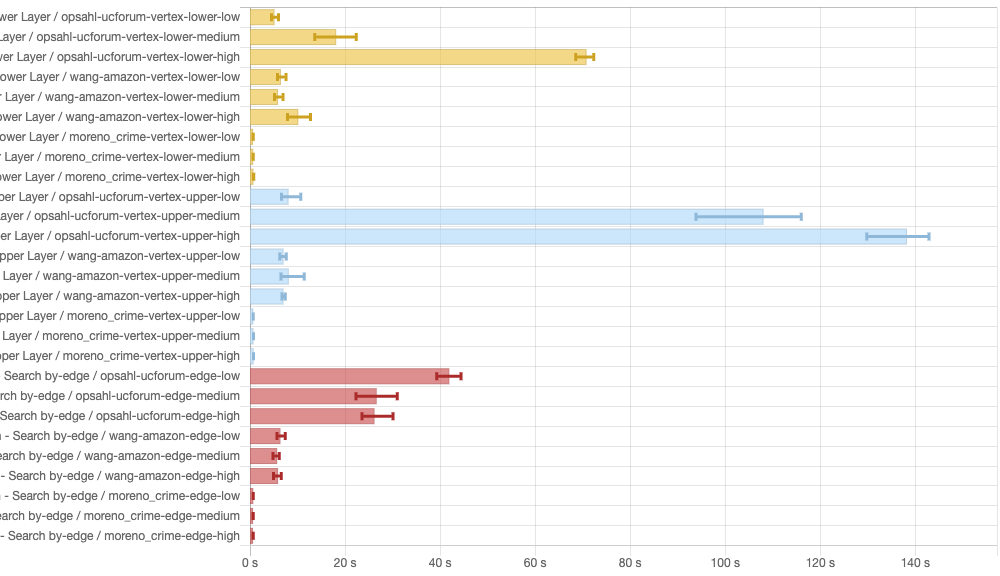
\includegraphics[width=\textwidth]{bench_1.png}
  \captionsetup{type=figure}
  \captionof{figure}{Benchmark 1 - DP in Haskell vs. Data.Graph Haskell}
  \label{fig:1}
\end{minipage}

\autoref{fig:1} shows that \acrshort{dpwcc} solution is $1.3$ faster compare with \acrshort{hs} \texttt{containers} library. Despite this, if we zoom  in \autoref{fig:1}, it can be observed that \acrshort{dpwcc} solution is slower compared with \acrshort{hs} \texttt{containers}; the reasons behind this have been explained in \autoref{sub:sec:e1}.
\iffalse
\begin{minipage}[t]{\linewidth}
  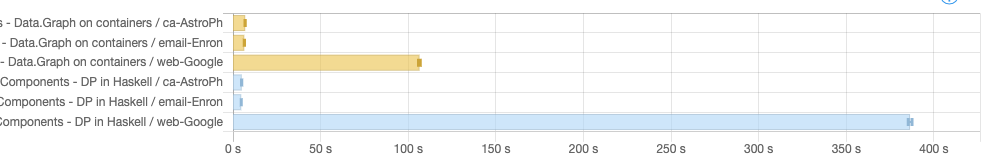
\includegraphics[width=\textwidth]{bench_2}
  \captionsetup{type=figure}
  \captionof{figure}{Benchmark 2 - DP in Haskell vs. Data.Graph Haskell}
  \label{fig:2}
\end{minipage}
\fi

Regarding mean execution times for each implementation on each case measure by \texttt{criterion} library \cite{criterion}, we can display the following results:

\begin{table}[H]
  \centering
  \begin{tabular}{|l|l|l|l|}
   \hline
   \textbf{Network} & \textbf{\acrshort{dpwcc}} & \textbf{\acrshort{hs} \texttt{containers}} & \textbf{Speed-up}\\
   \hline
   Enron Emails & 4.68s &  6.46s & 1.38\\
   \hline
   Astro Physics Coll Net & 4.98s & 6.95s  & 1.39\\
   \hline
   Google Web Graph & 386s & 106s & -3.64\\
   \hline
  \end{tabular}
 \caption{Mean Execution times}
 \label{table:6}
 \end{table}

These results allow for answering Question [Q2].
We already had a partial answer with the previous experiment E1 about [Q2] (\autoref{res:question}) where we have seen that the graph topology is affecting the performance and the parallelization, penalizing \acrshort{dpwcc} for this particular case. In this benchmark, the solution against a non-parallel \texttt{containers} \mintinline{haskell}{Data.Graph} confirms the hypothesis. 

\paragraph{Diefficency Metrics}\label{sub:sub:sec:e2}
Some considerations are needed before starting to analyze the data gathered with \acrshort{dm} tool. Firstly, the tool is plotting the results according to the traces generated by the implementation, both \acrshort{dpwcc} and \acrshort{hs} \emph{containers}. By the nature of \acrshort{dp} model, we can gather or register that timestamps as long as the model is generating results. In the case of \acrshort{hs} \texttt{containers}, this is not possible since it calculates \acrshort{wcc} at once. This is not an issue and we still can check at what point in time all \acrshort{wcc} in \acrshort{hs} \texttt{containers} are generated. In those cases, we are going to see a straight vertical line. 

It is important to remark that we needed to scale the timestamps because we have taken the time in nanoseconds. After all, the incremental generation between one \acrshort{wcc} and the other is very small but significant enough to be taken into consideration. Thus, if we left the time scale in integer milliseconds, microseconds, or nanoseconds integer part it cannot be appreciated. In case of escalation, we are discounting the nanosecond integer of the first generated results resulting in a time scale that starts close to $0$. This does not mean that the first result is generated at $0$ time, but we are discarding the previous time to focus on how the results are incrementally generated.

Having said that, we can see the results of \acrshort{dm} which are presented in two types of plots. The first one is regular line graphs in where the $x$ axis shows the time escalated when the result was generated and the $y$ axis is showing the component number that was generated at that time. The second type of plot is a radar plot in which shows how the solution is behaving on the dimensions of  \acrfull{tfft}, \acrfull{et}, \acrfull{tt}, \acrfull{comp} and \acrfull{dt} and how are the tension between them; all these metrics are higher is better. All the details about these metrics are explained here \cite{diefpaper}.

\begin{figure}[!htb]
    \centering
    \begin{minipage}{0.33\textwidth}
     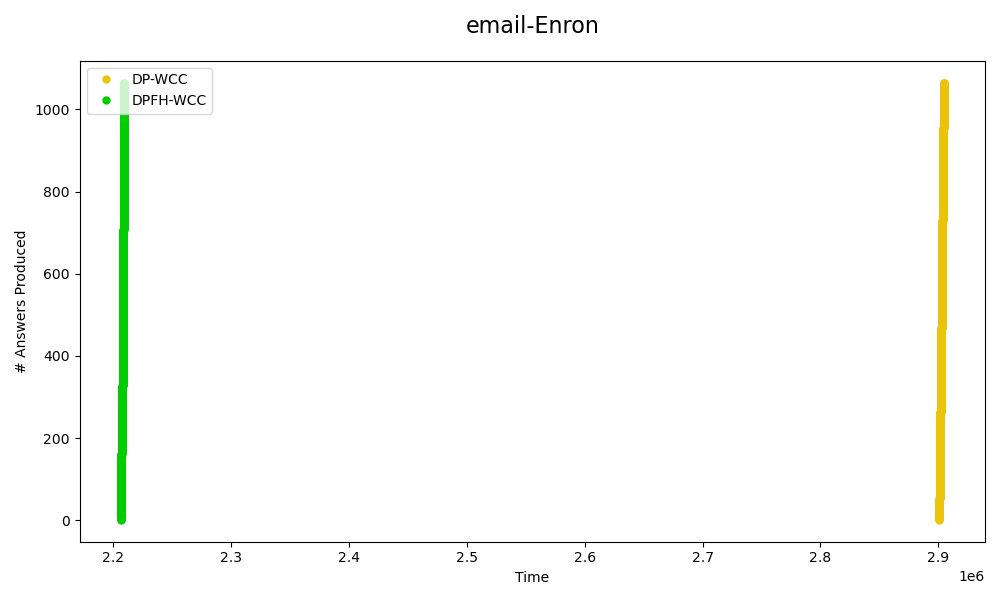
\includegraphics[width=1\linewidth, height=0.2\textheight]{email_enron}
      \caption{email-Enron \acrshort{dm}}
      \label{fig:dief:1}
    \end{minipage}%
    \begin{minipage}{0.33\textwidth}
     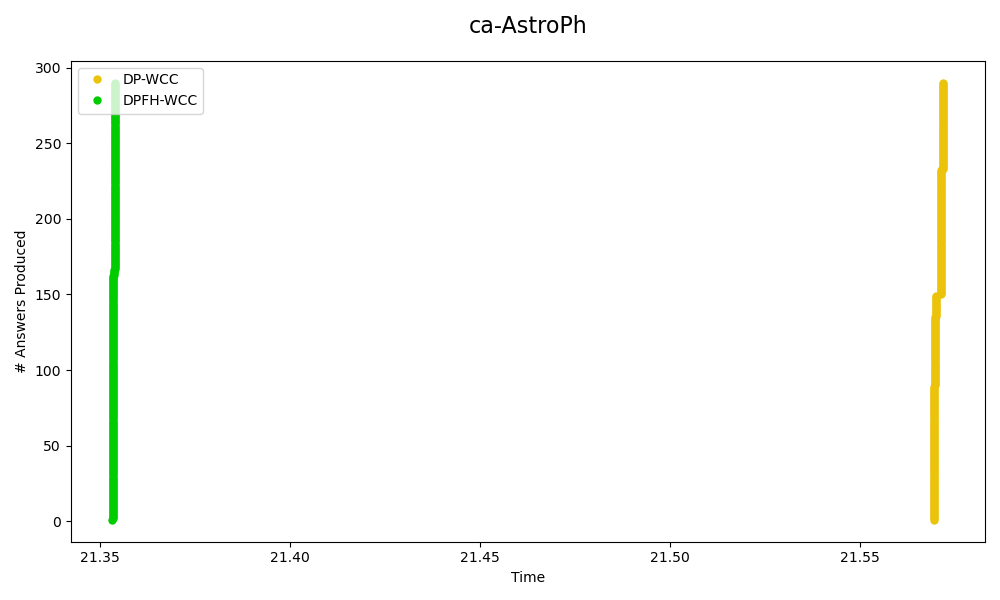
\includegraphics[width=1\linewidth, height=0.2\textheight]{ca_astroph}
      \caption{ca-AstroPh \acrshort{dm}}
      \label{fig:dief:2}
    \end{minipage}%
    \begin{minipage}{0.33\textwidth}
     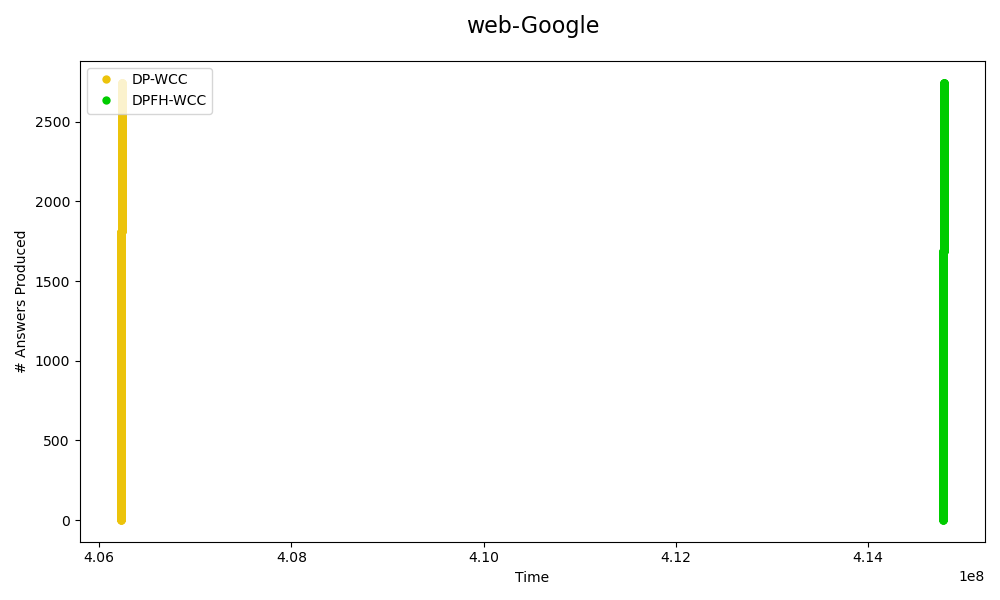
\includegraphics[width=1\linewidth, height=0.2\textheight]{web_google}
      \caption{web-Google \acrshort{dm}}
      \label{fig:dief:3}
    \end{minipage}
\end{figure}

Based on the results shown in all the figures above, all the solutions in \acrshort{dpwcc} are being generated incrementally, but there is some difference that we would like to remark. In the case of \emph{email-Enron} and \emph{ca-AstroPh} graphs as we can see in \autoref{fig:dief:1} and \autoref{fig:dief:2}, there seems to be a more incremental generation of results. This is behavior is measured with the values of \acrfull{dt}. \emph{ca-AstroPh} as it can be seen in \autoref{fig:dief:2}, is even more incremental showing a clear separation between some results and others. The \emph{web-Google} network which is shown in \autoref{fig:dief:3}, is a little more linear and that is because all the results are being generated with very little difference in time between them. This is due to the fact of the explained reasons in \autoref{sub:sec:e1}. Having the biggest \acrshort{wcc} at the end of \emph{web-Google} \acrshort{dp} algorithm it is retaining results until the biggest \acrshort{wcc} can be solved, which takes longer. 

\begin{figure}[!htb]
    \centering
    \begin{minipage}{0.33\textwidth}
     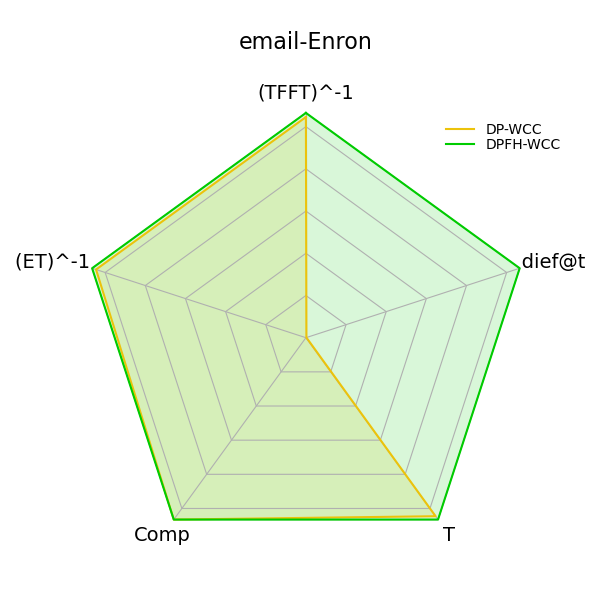
\includegraphics[width=1\linewidth, height=0.2\textheight]{email_enron_radar}
      \caption{email-Enron \acrshort{dm}}
      \label{fig:dief:rad:1}
    \end{minipage}%
    \begin{minipage}{0.33\textwidth}
     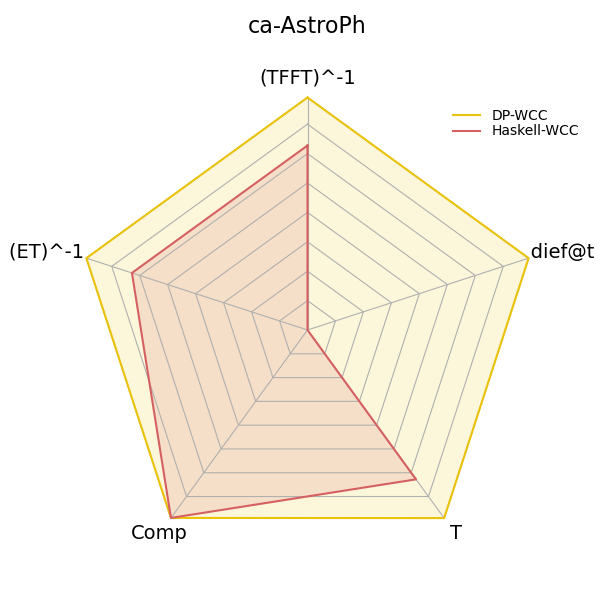
\includegraphics[width=1\linewidth, height=0.2\textheight]{ca_astroph_radar}
      \caption{ca-AstroPh \acrshort{dm}}
      \label{fig:dief:rad:2}
    \end{minipage}%
    \begin{minipage}{0.33\textwidth}
     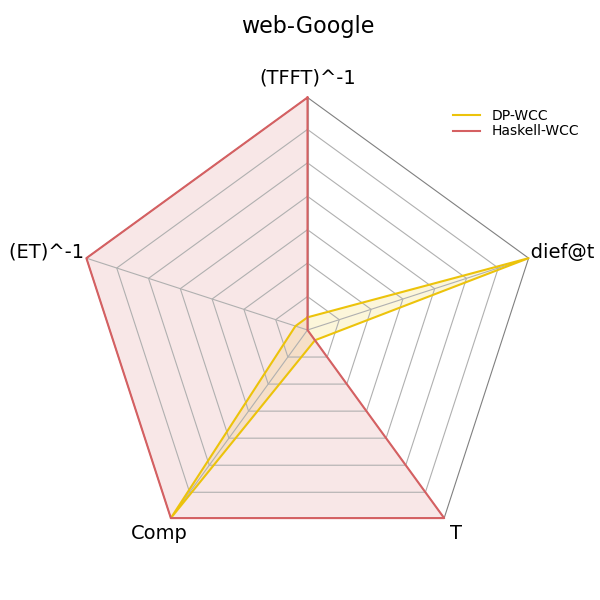
\includegraphics[width=1\linewidth, height=0.2\textheight]{web_google_radar}
      \caption{web-Google \acrshort{dm}}
      \label{fig:dief:rad:3}
    \end{minipage}
\end{figure}

As we can appreciate in the above radar plots our previous analysis can be confirmed. We can see for example that the \acrlong{tt} of \emph{web-Google} in \autoref{fig:dief:rad:3}, in the case of \acrshort{dpwcc} is worse than \acrshort{hs} \texttt{containers}, which is not happening for the others.

In conclusion, we can say that regarding [Q2] (\autoref{res:question}) although \acrshort{dpwcc} is faster than the traditional approach, the speed-up dimension execution factor is not always the most interest analysis that we can have, because as we have seen even when in the case of \emph{web-Google} Graph \acrshort{dpwcc} is slower at execution, it is at least generating incremental results without the need to wait for the rest of the computations.

\subsection{Experiment: E3}
For this type of analysis, our experiment focuses on \emph{email-Enron} network \cite{netenron} only because profiling data generated by \acrshort{ghc} is big enough to conduct the analysis and on the other, and enabling profiling penalize execution time.

\paragraph{Multithreading} For analyzing parallelization and multithreading we have used \textit{ThreadScope} \cite{threadscope} which allows us to see how the parallelization is taking place on \acrshort{ghc} at a fine grained level and how the threads are distributed throughout the different cores requested with the \mintinline{bash}{-N} execution \texttt{ghc-option} flag.

\begin{minipage}[t!]{\linewidth}

  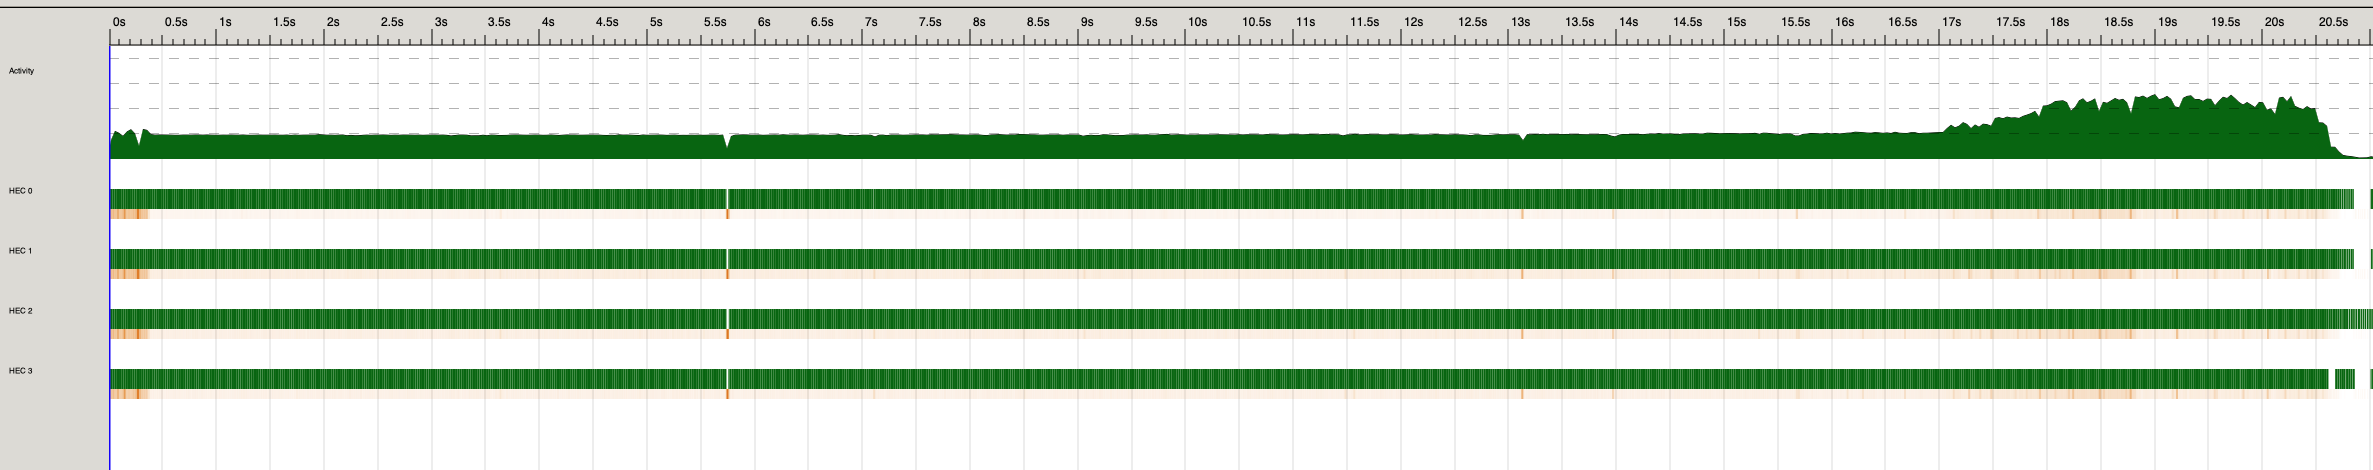
\includegraphics[width=\textwidth]{screen_1}
  \captionsetup{type=figure}
  \captionof{figure}{Threadscope Image of General Execution}
  \label{fig:3}
\end{minipage}

In \autoref{fig:3}, we can see that the parallelization is being distributed evenly among the $4$ Cores that we have set for this execution.
The distribution of the load is more intensive at the end of the execution, where \mintinline{haskell}{actor2} filter stage 
%as it can be seen in \autoref{src:haskell:3}, 
of the algorithm is taking place and different filters are reaching execution of that second actor.

\begin{wrapfigure}{r}{0.5\textwidth}
  \begin{center}
     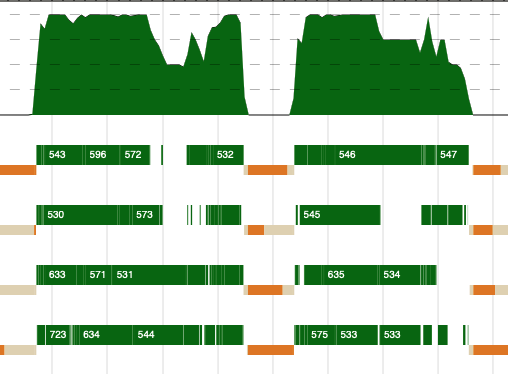
\includegraphics[width=0.48\textwidth] {screen_2}
     %[width=10cm, height=9cm]
       \end{center}
     \caption{Threadscope Image of Zoomed Fraction}
     \label{fig:4}
 %\end{figure}
 \end{wrapfigure}
Another important aspect shown in \autoref{fig:3}, is that this work is not so significant for \acrshort{ghc} and the threads and distribution of the work keeps between 1 or 2 cores during the execution time of the \mintinline{haskell}{actor1}. However, the usages increase on the second actor as pointed out before. In this regard, we can answer research questions [Q1] and [Q3] (\autoref{res:question}), verifying that \acrshort{hs} not only supports the required parallelization level but is evenly distributed across the program execution too.

Finally, it can also be appreciated that there is no sequential execution on any part of the program because the $4$ cores have \textit{CPU} activity during the whole execution time. This is because as long the program start, and because of the nature of the \acrshort{dp} model, it is spawning the \textit{Source} stage in a separated thread. This is a clear advantage for the model and the processing of the data since the program does not need to wait to do some sequential processing like reading a file, before start computing the rest of the stages.




%\begin{minipage}[t!]{\linewidth}
%\begin{center}
%  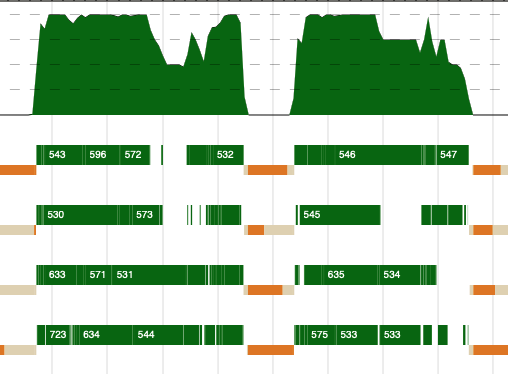
\includegraphics[width=0.6\textwidth]{screen_2}
%  \captionsetup{type=figure}
%  \captionof{figure}{Threadscope Image of Zoomed Fraction}
%  \label{fig:4}
%  \end{center}
%\end{minipage}

\autoref{fig:4} zooms in on \textit{ThreadScope} output in a particular moment, approximately in the middle of the execution. We can appreciate how many threads are being spawned and by the tool and if they are evenly distributed among cores. The numbers inside green bars represent the number of threads that are being executed on that particular core (horizontal line) at that execution slot. Thus, the number of threads varies among slot execution times because as it is already known, \acrshort{ghc} implements \emph{Preemptive Scheduling} \cite{lightweightghc}.

Having said that, it can be appreciated in \autoref{fig:4} our first assumption that the load is evenly distributed because the mean number of executing threads per core is $571$.

\paragraph{Memory allocation} Another important aspect in our case is how the memory is being managed to avoid memory leaks or other non-desired behavior that increases memory allocation during the execution time. This is even more important in the particular implementation of \acrshort{wcc} using \acrshort{dp} model because it requires to maintain the set of connected components in memory throughout the execution of the program or at least until we can output the calculated \acrshort{wcc} if we reach to the last \textit{Filter} and we know that this \acrshort{wcc} cannot be enlarged anymore. 

In order to verify this, we measure memory allocation with \textit{eventlog2html} \cite{eventlog2html} which converts generated profiling memory eventlog files into graphical HTML representation. 

\begin{wrapfigure}{r}{0.5\textwidth}
  \begin{center}
     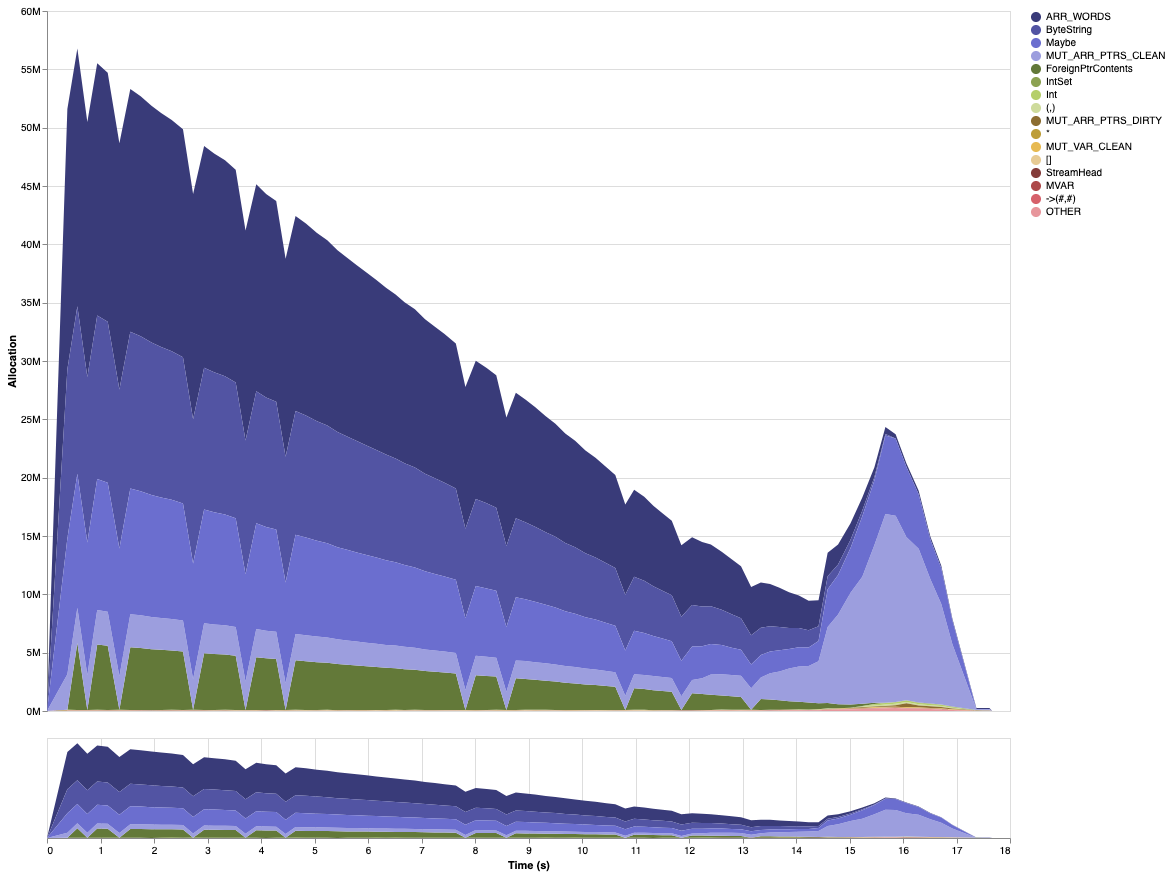
\includegraphics[width=0.5\textwidth] {visualization}
     %[width=10cm, height=9cm]
       \end{center}
     \caption{Memory Allocation}
     \label{fig:5}
 %\end{figure}
 \end{wrapfigure}
 
%\begin{minipage}[t]{\linewidth}
%\begin{center}
%  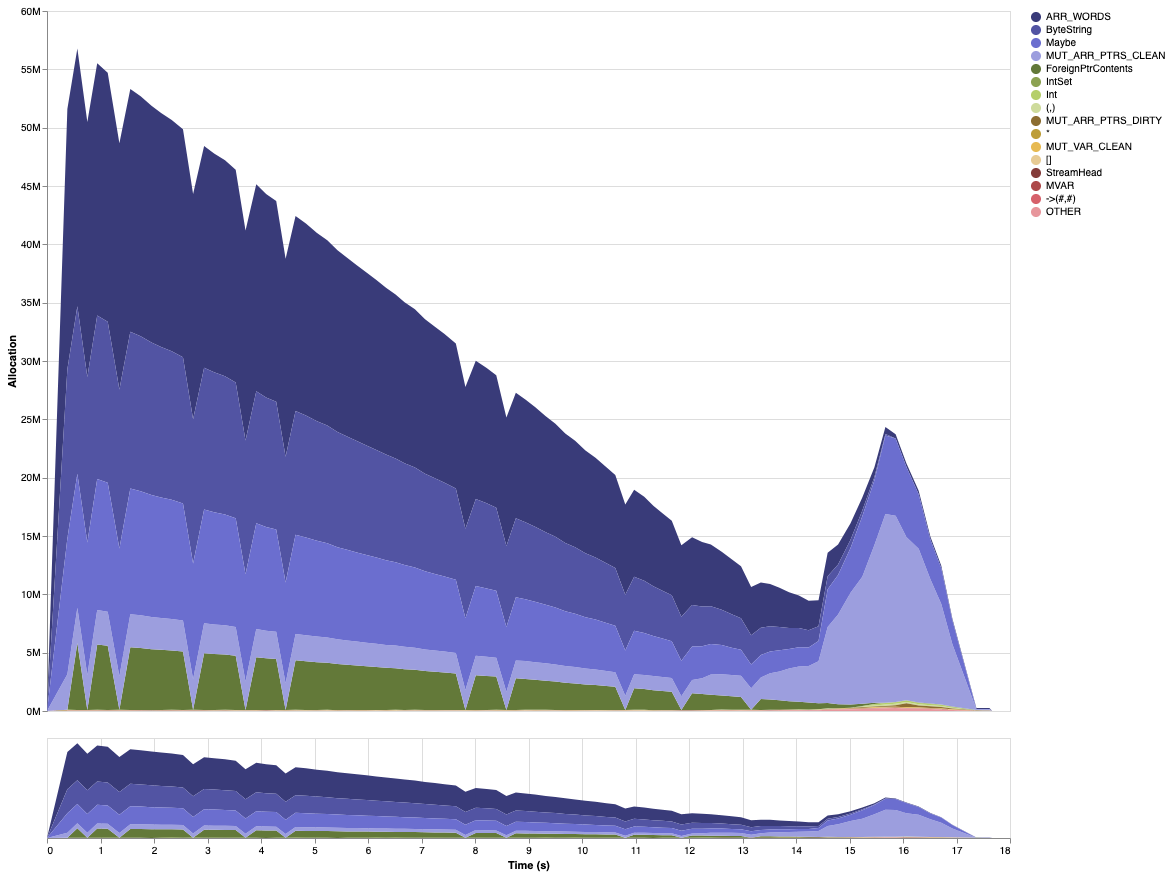
\includegraphics[width=0.6\textwidth]{visualization}
%  \captionsetup{type=figure}
%  \captionof{figure}{Memory Allocation}
%  \label{fig:5}
%  \end{center}
%\end{minipage}

As we can see in \autoref{fig:5}, \acrshort{dpwcc} does an efficient work on allocating memory since we are not using more than $57$ MB of memory during the whole execution of the program.

On the other hand, if we analyze how the memory is allocated during the execution of the program, it can also be appreciated that most of the memory is allocated at the beginning of the program and steadily decrease over time with a small peak at the end that does not overpass even half of the initial peak of $57$ MB. The explanation for this behavior is quite straightforward because at the beginning we are reading from the file and transforming a \mintinline{haskell}{ByteString} buffer to \mintinline{haskell}{(Int, Int)} edges. This is seen in the image in which the dark blue that is on top of the area is \mintinline{haskell}{ByteString} allocation. Light blue is allocation of \mintinline{haskell}{Maybe a} type which is the type that is returned by the \textit{Channels} because it can contain a value or not. Data value \mintinline{haskell}{Nothing} is indicating end of the \textit{Channel}. 
%as we can see in \autoref{src:haskell:f3}.

Another important aspect is the green area which represents \mintinline{haskell}{IntSet} allocation, which in the case of our program is the data structure that we use to gather the set of vertices that represents a \acrshort{wcc}. This means that the amount of memory used for gathering the \acrshort{wcc} itself is minimum and it is decreasing over time, which is another empirical indication that we are incrementally releasing results to the user. It can be seen as well that as long the green area reduces the lighter blue (\mintinline{haskell}{MUT_ARR_PTRS_CLEAN} \cite{ghcheap}) increases at the same time indicating that the computations for the output (releasing results) is taking place. 

Finally, according to what we have stated above, we can answer the question [Q3] (\autoref{res:question}) showing that not only memory management was efficient, but at the same time, the memory was not leaking or increasing across the running execution program.


